\section{Video Conferencing}
As part of deliverables for our final year project, we offer a video conferencing solution which aims to operate at 
lower internet bandwidth connections, by utilising a neural network-based video compression technique. 
However, for the scope of our project, we produced a proof of concept of the neural network, and a video 
conferencing platform without neural network integration.

We focussed on two ways going about developing a video conferencing solution, one being a ground-up approach using peer 
to peer communication(Mesh) using webRTC and the other one using a pre-built video conferencing API’s of Jitsi 
(an open-source video conferencing software).

\subsection{Thought process}

The reason to go for a ground-up approach or an open-source solution was to be able to access the entire code 
base and therefore be able to integrate our neural network compression technique in the future and also to be able to
customize the user interface for varied business needs and setups.

% ref(PeerJS documentation): https://peerjs.com/docs.html#peerconnect-options
% ref(socket.io documentation): https://socket.io/docs/v4/index.html
\subsection{ Peer to Peer with webRTC and Mesh approach}
In a peer-to-peer connection, one client communicates with another client directly after minimal or no communication with a central server.
For multiple clients though, it becomes necessary to have a central server managing all the connections of clients.
One approach of using peer-to-peer communication for multiple users/clients is a Mesh approach in which each client sends and receives data streams to and from all the other clients in a room.
Even though there exist better approaches towards video conferencing including the SFU (Simple Forwarding Unit), 
mesh approach would give us a worst-case scenario to test out our neural network solution and would become a benchmark for other approaches.

\begin{figure}
    \begin{center}
        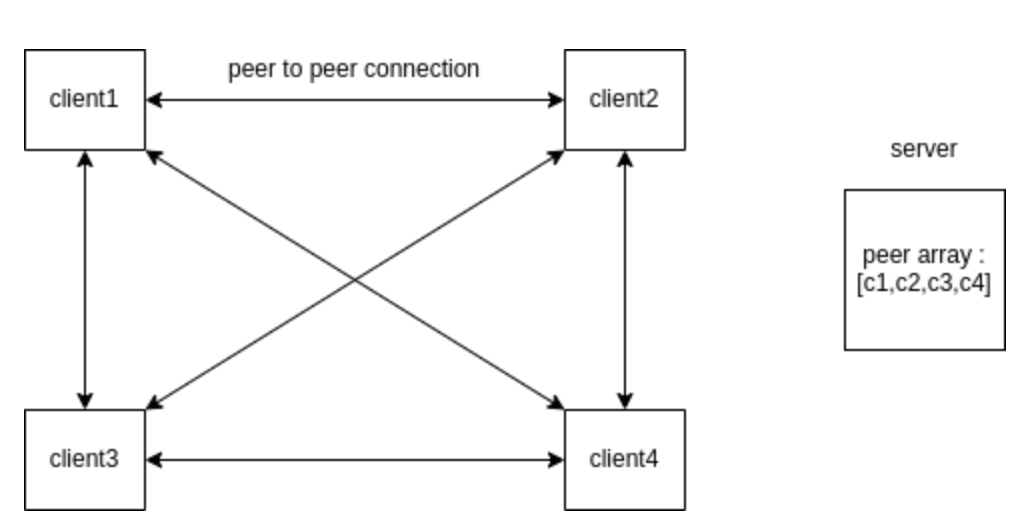
\includegraphics[width=15cm]{p2pMesh.png}
    \end{center}
    \caption{WebRTC Mesh video conferencing system.}
    \label{fig:p2pMesh}
\end{figure}

\begin{itemize}
    \item The mesh consists of all the clients connected to all the other clients in a peer-to-peer connection transferring data 1:1.
    \item The server does the initial connection set up amongst the peer clients and maintains an array of all the active peers/clients.
    \item Clients request the server for a connection with all the other active clients in a room to which the server responds by looping through the peer array and setting up a connection for each.
    \item User Interface can be developed and customized fully.
\end{itemize}

\subsubsection{Pros}

\begin{itemize}
    \item Full freedom to develop a platform with no limits on functionality.
    \item No dependency on an external API which may change over time.
    \item Simple approach to testing out the neural network.
\end{itemize}

\subsubsection{Cons}

\begin{itemize}
    \item The Mesh approach needs a lot of resources and cannot handle many participants.
    \item Needs a better server machine to handle more clients with ease.
    \item Developing functionalities and testing them for security may become time-consuming.
\end{itemize}

% ref(jitsi IFrame api): https://jitsi.github.io/handbook/docs/dev-guide/dev-guide-iframe
% ref(jitsi lib-jitsi-meet api): https://github.com/jitsi/lib-jitsi-meet 
\subsection{Jitsi API}
Jitsi is an open-source video conferencing platform, which can be hosted locally and is customizable using Jitsi API libraries.
Extra authentication of the users concerning the hosting app can be added using techniques like JWT authentication.

%refrecre for image: https://jitsi.github.io/handbook/docs/devops-guide/devops-guide-docker
\begin{figure}[h!]
    \begin{center}
        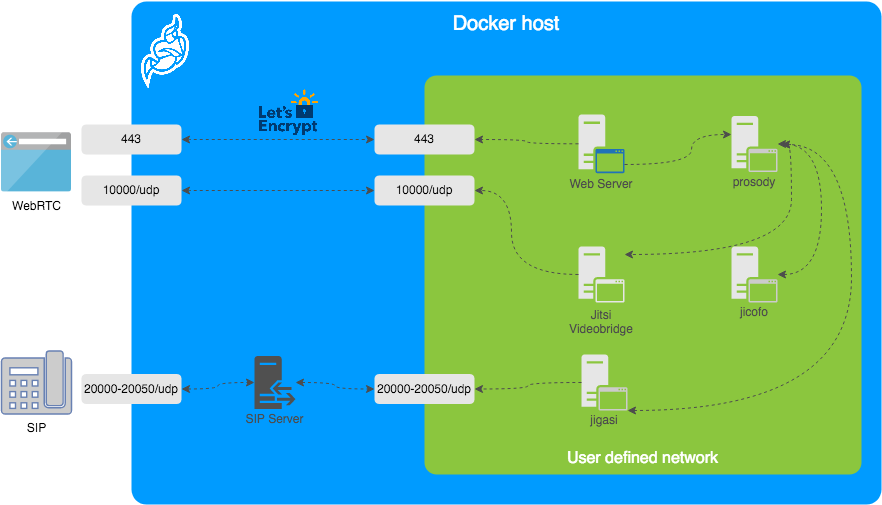
\includegraphics[width=15cm]{docker-jitsi-meet.png}
    \end{center}
    \caption{Jitsi meet services.}
    \label{fig:jitsimeet}
\end{figure}

\begin{itemize}
    \item  Jitsi comprises of Jitsi Meet which is a WebRTC compatible javascript application that uses Video bridge to provide high quality, scalable video conferences.
    \item Video bridge is a WebRTC compatible server designed to route video streams amongst participants in a conference.
    \item jicofo(Jitsi Conference Focus) manages media sessions and acts as a load balancer.
    \item Jitsi SIP is not included as it is out of the scope of this project.
\end{itemize}

\subsubsection{Pros}

\begin{itemize}
    \item Integrable as an IFrame in an already existing app.
    \item Provides security, more functionality, and customizability.
    \item Easier to set up with the publicly accessible server of jitsi.
\end{itemize}

\subsubsection{Cons}

\begin{itemize}
    \item Limited UI customizability with Jitsi IFrame API.
    \item Slower or laggy service if using the public server or a server with less processing power.
    \item High learning curve if setting up a server locally.
\end{itemize}